% Options for packages loaded elsewhere
\PassOptionsToPackage{unicode}{hyperref}
\PassOptionsToPackage{hyphens}{url}
%
\documentclass[
]{article}
\usepackage{amsmath,amssymb}
\usepackage{iftex}
\ifPDFTeX
  \usepackage[T1]{fontenc}
  \usepackage[utf8]{inputenc}
  \usepackage{textcomp} % provide euro and other symbols
\else % if luatex or xetex
  \usepackage{unicode-math} % this also loads fontspec
  \defaultfontfeatures{Scale=MatchLowercase}
  \defaultfontfeatures[\rmfamily]{Ligatures=TeX,Scale=1}
\fi
\usepackage{lmodern}
\ifPDFTeX\else
  % xetex/luatex font selection
\fi
% Use upquote if available, for straight quotes in verbatim environments
\IfFileExists{upquote.sty}{\usepackage{upquote}}{}
\IfFileExists{microtype.sty}{% use microtype if available
  \usepackage[]{microtype}
  \UseMicrotypeSet[protrusion]{basicmath} % disable protrusion for tt fonts
}{}
\makeatletter
\@ifundefined{KOMAClassName}{% if non-KOMA class
  \IfFileExists{parskip.sty}{%
    \usepackage{parskip}
  }{% else
    \setlength{\parindent}{0pt}
    \setlength{\parskip}{6pt plus 2pt minus 1pt}}
}{% if KOMA class
  \KOMAoptions{parskip=half}}
\makeatother
\usepackage{xcolor}
\usepackage[margin=1in]{geometry}
\usepackage{color}
\usepackage{fancyvrb}
\newcommand{\VerbBar}{|}
\newcommand{\VERB}{\Verb[commandchars=\\\{\}]}
\DefineVerbatimEnvironment{Highlighting}{Verbatim}{commandchars=\\\{\}}
% Add ',fontsize=\small' for more characters per line
\usepackage{framed}
\definecolor{shadecolor}{RGB}{248,248,248}
\newenvironment{Shaded}{\begin{snugshade}}{\end{snugshade}}
\newcommand{\AlertTok}[1]{\textcolor[rgb]{0.94,0.16,0.16}{#1}}
\newcommand{\AnnotationTok}[1]{\textcolor[rgb]{0.56,0.35,0.01}{\textbf{\textit{#1}}}}
\newcommand{\AttributeTok}[1]{\textcolor[rgb]{0.13,0.29,0.53}{#1}}
\newcommand{\BaseNTok}[1]{\textcolor[rgb]{0.00,0.00,0.81}{#1}}
\newcommand{\BuiltInTok}[1]{#1}
\newcommand{\CharTok}[1]{\textcolor[rgb]{0.31,0.60,0.02}{#1}}
\newcommand{\CommentTok}[1]{\textcolor[rgb]{0.56,0.35,0.01}{\textit{#1}}}
\newcommand{\CommentVarTok}[1]{\textcolor[rgb]{0.56,0.35,0.01}{\textbf{\textit{#1}}}}
\newcommand{\ConstantTok}[1]{\textcolor[rgb]{0.56,0.35,0.01}{#1}}
\newcommand{\ControlFlowTok}[1]{\textcolor[rgb]{0.13,0.29,0.53}{\textbf{#1}}}
\newcommand{\DataTypeTok}[1]{\textcolor[rgb]{0.13,0.29,0.53}{#1}}
\newcommand{\DecValTok}[1]{\textcolor[rgb]{0.00,0.00,0.81}{#1}}
\newcommand{\DocumentationTok}[1]{\textcolor[rgb]{0.56,0.35,0.01}{\textbf{\textit{#1}}}}
\newcommand{\ErrorTok}[1]{\textcolor[rgb]{0.64,0.00,0.00}{\textbf{#1}}}
\newcommand{\ExtensionTok}[1]{#1}
\newcommand{\FloatTok}[1]{\textcolor[rgb]{0.00,0.00,0.81}{#1}}
\newcommand{\FunctionTok}[1]{\textcolor[rgb]{0.13,0.29,0.53}{\textbf{#1}}}
\newcommand{\ImportTok}[1]{#1}
\newcommand{\InformationTok}[1]{\textcolor[rgb]{0.56,0.35,0.01}{\textbf{\textit{#1}}}}
\newcommand{\KeywordTok}[1]{\textcolor[rgb]{0.13,0.29,0.53}{\textbf{#1}}}
\newcommand{\NormalTok}[1]{#1}
\newcommand{\OperatorTok}[1]{\textcolor[rgb]{0.81,0.36,0.00}{\textbf{#1}}}
\newcommand{\OtherTok}[1]{\textcolor[rgb]{0.56,0.35,0.01}{#1}}
\newcommand{\PreprocessorTok}[1]{\textcolor[rgb]{0.56,0.35,0.01}{\textit{#1}}}
\newcommand{\RegionMarkerTok}[1]{#1}
\newcommand{\SpecialCharTok}[1]{\textcolor[rgb]{0.81,0.36,0.00}{\textbf{#1}}}
\newcommand{\SpecialStringTok}[1]{\textcolor[rgb]{0.31,0.60,0.02}{#1}}
\newcommand{\StringTok}[1]{\textcolor[rgb]{0.31,0.60,0.02}{#1}}
\newcommand{\VariableTok}[1]{\textcolor[rgb]{0.00,0.00,0.00}{#1}}
\newcommand{\VerbatimStringTok}[1]{\textcolor[rgb]{0.31,0.60,0.02}{#1}}
\newcommand{\WarningTok}[1]{\textcolor[rgb]{0.56,0.35,0.01}{\textbf{\textit{#1}}}}
\usepackage{graphicx}
\makeatletter
\def\maxwidth{\ifdim\Gin@nat@width>\linewidth\linewidth\else\Gin@nat@width\fi}
\def\maxheight{\ifdim\Gin@nat@height>\textheight\textheight\else\Gin@nat@height\fi}
\makeatother
% Scale images if necessary, so that they will not overflow the page
% margins by default, and it is still possible to overwrite the defaults
% using explicit options in \includegraphics[width, height, ...]{}
\setkeys{Gin}{width=\maxwidth,height=\maxheight,keepaspectratio}
% Set default figure placement to htbp
\makeatletter
\def\fps@figure{htbp}
\makeatother
\setlength{\emergencystretch}{3em} % prevent overfull lines
\providecommand{\tightlist}{%
  \setlength{\itemsep}{0pt}\setlength{\parskip}{0pt}}
\setcounter{secnumdepth}{-\maxdimen} % remove section numbering
\ifLuaTeX
  \usepackage{selnolig}  % disable illegal ligatures
\fi
\usepackage{bookmark}
\IfFileExists{xurl.sty}{\usepackage{xurl}}{} % add URL line breaks if available
\urlstyle{same}
\hypersetup{
  pdftitle={CodingChallenge\_DataWrangling},
  pdfauthor={Vaibhav B. Shelar},
  hidelinks,
  pdfcreator={LaTeX via pandoc}}

\title{CodingChallenge\_DataWrangling}
\author{Vaibhav B. Shelar}
\date{2025-03-23}

\begin{document}
\maketitle

\begin{Shaded}
\begin{Highlighting}[]
\FunctionTok{library}\NormalTok{(tidyverse)}
\end{Highlighting}
\end{Shaded}

\begin{verbatim}
## -- Attaching core tidyverse packages ------------------------ tidyverse 2.0.0 --
## v dplyr     1.1.4     v readr     2.1.5
## v forcats   1.0.0     v stringr   1.5.1
## v ggplot2   3.5.1     v tibble    3.2.1
## v lubridate 1.9.4     v tidyr     1.3.1
## v purrr     1.0.4     
## -- Conflicts ------------------------------------------ tidyverse_conflicts() --
## x dplyr::filter() masks stats::filter()
## x dplyr::lag()    masks stats::lag()
## i Use the conflicted package (<http://conflicted.r-lib.org/>) to force all conflicts to become errors
\end{verbatim}

\begin{Shaded}
\begin{Highlighting}[]
\DocumentationTok{\#\#\# Q2}

\CommentTok{\# load csv file}

\NormalTok{diversity\_data }\OtherTok{\textless{}{-}} \FunctionTok{read.csv}\NormalTok{(}\StringTok{"DiversityData.csv"}\NormalTok{)}

\NormalTok{meta\_data }\OtherTok{\textless{}{-}} \FunctionTok{read.csv}\NormalTok{(}\StringTok{"Metadata.csv"}\NormalTok{)}

\CommentTok{\# join the dataframe by the common column}

\NormalTok{alpha }\OtherTok{\textless{}{-}} \FunctionTok{left\_join}\NormalTok{(diversity\_data, meta\_data, }\AttributeTok{by =} \StringTok{"Code"}\NormalTok{)}
\end{Highlighting}
\end{Shaded}

\begin{Shaded}
\begin{Highlighting}[]
\DocumentationTok{\#\#\# Q3}

\CommentTok{\# a)}

\FunctionTok{library}\NormalTok{(dplyr)}

\CommentTok{\# calculating Pielou\textquotesingle{}s evenness index}

\NormalTok{alpha}\SpecialCharTok{$}\NormalTok{Pielou\_evenness }\OtherTok{\textless{}{-}} \FunctionTok{log}\NormalTok{(alpha}\SpecialCharTok{$}\NormalTok{richness)}

\CommentTok{\# Create a new column called Pielou\_evenness and name the dataframe as alpha\_even}
\NormalTok{alpha\_even }\OtherTok{\textless{}{-}}\NormalTok{ alpha }\SpecialCharTok{\%\textgreater{}\%}
              \FunctionTok{mutate}\NormalTok{(}\AttributeTok{Pielou\_evenness =}\NormalTok{ shannon }\SpecialCharTok{/} \FunctionTok{log}\NormalTok{(richness))}
\end{Highlighting}
\end{Shaded}

\subsubsection{Q4}\label{q4}

\begin{Shaded}
\begin{Highlighting}[]
\CommentTok{\# summarizing Pielou\textquotesingle{}s evenness by Crop and Time\_Point and Summarize the data}

\NormalTok{alpha\_average }\OtherTok{\textless{}{-}}\NormalTok{ alpha\_even }\SpecialCharTok{\%\textgreater{}\%}
                  \FunctionTok{group\_by}\NormalTok{(Crop, Time\_Point) }\SpecialCharTok{\%\textgreater{}\%}
                  \FunctionTok{summarise}\NormalTok{(}\AttributeTok{mean\_even =} \FunctionTok{mean}\NormalTok{(Pielou\_evenness),}
                  \AttributeTok{count\_even =} \FunctionTok{n}\NormalTok{(),}
                  \AttributeTok{sd.dev =} \FunctionTok{sd}\NormalTok{(Pielou\_evenness),}
                  \AttributeTok{sd.err =} \FunctionTok{sd}\NormalTok{(Pielou\_evenness)}\SpecialCharTok{/}\FunctionTok{sqrt}\NormalTok{(}\FunctionTok{n}\NormalTok{()))}
\end{Highlighting}
\end{Shaded}

\begin{verbatim}
## `summarise()` has grouped output by 'Crop'. You can override using the
## `.groups` argument.
\end{verbatim}

\subsubsection{Q5}\label{q5}

\section{Calculate the difference between the soybean column, the soil
column, and the difference between the cotton column and the soil
column}\label{calculate-the-difference-between-the-soybean-column-the-soil-column-and-the-difference-between-the-cotton-column-and-the-soil-column}

\begin{Shaded}
\begin{Highlighting}[]
\NormalTok{alpha\_average2 }\OtherTok{\textless{}{-}}\NormalTok{ alpha\_average }\SpecialCharTok{\%\textgreater{}\%}
                  \FunctionTok{select}\NormalTok{(Time\_Point, Crop, mean\_even) }\SpecialCharTok{\%\textgreater{}\%}
                  \FunctionTok{pivot\_wider}\NormalTok{(}\AttributeTok{names\_from =}\NormalTok{ Crop, }\AttributeTok{values\_from =}\NormalTok{ mean\_even) }\SpecialCharTok{\%\textgreater{}\%}
                  \FunctionTok{mutate}\NormalTok{(}\AttributeTok{diff.cotton.even =}\NormalTok{ Soil }\SpecialCharTok{{-}}\NormalTok{ Cotton,}
                         \AttributeTok{diff.soybean.even =}\NormalTok{ Soil }\SpecialCharTok{{-}}\NormalTok{ Soybean)}
\end{Highlighting}
\end{Shaded}

\subsubsection{Q6}\label{q6}

\section{Connecting it to plots}\label{connecting-it-to-plots}

\begin{Shaded}
\begin{Highlighting}[]
\NormalTok{alpha\_average2 }\SpecialCharTok{\%\textgreater{}\%}
  \FunctionTok{select}\NormalTok{(Time\_Point, diff.cotton.even, diff.soybean.even) }\SpecialCharTok{\%\textgreater{}\%}  \CommentTok{\# Select relevant columns}
  \FunctionTok{pivot\_longer}\NormalTok{(}\AttributeTok{cols =} \FunctionTok{c}\NormalTok{(diff.cotton.even, diff.soybean.even), }\AttributeTok{names\_to =} \StringTok{"diff"}\NormalTok{) }\SpecialCharTok{\%\textgreater{}\%}
  \FunctionTok{ggplot}\NormalTok{(}\FunctionTok{aes}\NormalTok{(}\AttributeTok{x =}\NormalTok{ Time\_Point, }\AttributeTok{y =}\NormalTok{ value, }\AttributeTok{color =}\NormalTok{ diff)) }\SpecialCharTok{+}
  \FunctionTok{geom\_line}\NormalTok{(}\AttributeTok{size =} \DecValTok{1}\NormalTok{) }\SpecialCharTok{+}  \CommentTok{\# Line plot}
  \FunctionTok{theme\_minimal}\NormalTok{() }\SpecialCharTok{+}  \CommentTok{\# Clean theme}
  \FunctionTok{labs}\NormalTok{(}
    \AttributeTok{x =} \StringTok{"Time (hrs)"}\NormalTok{,}
    \AttributeTok{y =} \StringTok{"Difference from soil in Pielou’s evenness"}\NormalTok{,}
    \AttributeTok{color =} \StringTok{"diff"}
\NormalTok{  ) }\SpecialCharTok{+} 
  \FunctionTok{theme}\NormalTok{(}\AttributeTok{legend.position =} \StringTok{"right"}\NormalTok{)}
\end{Highlighting}
\end{Shaded}

\begin{verbatim}
## Warning: Using `size` aesthetic for lines was deprecated in ggplot2 3.4.0.
## i Please use `linewidth` instead.
## This warning is displayed once every 8 hours.
## Call `lifecycle::last_lifecycle_warnings()` to see where this warning was
## generated.
\end{verbatim}

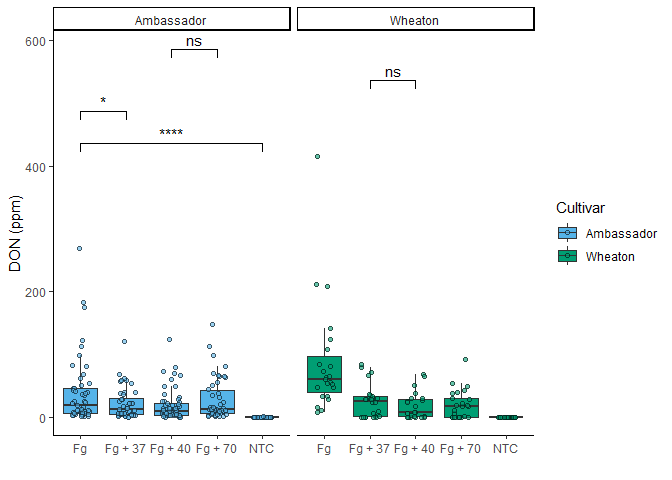
\includegraphics{CodingChallenge_DataWrangling_files/figure-latex/unnamed-chunk-6-1.pdf}

\end{document}
